\def \title{bladeRF User Guide}
\def \subtitle{A comprehensive user guide for the Nuand bladeRF}

% Author email and affiliation
\def \emailbpadalino    {\href{mailto:brian.padalino@nuand.com?cc=bladeRF@nuand.com}{\textless{brian.padalino@nuand.com}\textgreater}}
\def \emailjszymaniak   {\href{mailto:jon.szymaniak@nuand.com?cc=bladeRF@nuand.com}{\textless{jon.szymaniak@nuand.com}\textgreater}}
\def \afilnuand         {Nuand, LLC}

% Define authors table
\def \authors{
  \begin{table}[h]
    \centering
    \begin{tabular}{cc}
      Brian Padalino    & Jon Szymaniak     \\
      \emailbpadalino   & \emailjszymaniak  \\
      \afilnuand        & \afilnuand        \\
    \end{tabular}
  \end{table}
}

% Contributors table
%\def \contributors{
%  \begin{table}[h]
%    \centering
%    \begin{tabular}{c}
%    \end{tabular}
%  \end{table}
%}

\def \tablerowcolor{\rowcolor[HTML]{C0C0C0}}
\def \tablecolcolor{\columncolor[HTML]{C0C0C0}}

\def \revisions {
  \begin{table}[h]
    \centering
    \begin{tabular}{|c|c|l|}
      \hline
      \tablerowcolor
      \textbf{Revision} & \textbf{Date} & \textbf{Summary} \hspace{4in}  \\ \hline
      1  & TBD & Draft: Work in progress \\ \hline
    \end{tabular}
  \end{table}
}

% Enable Figure and Table index
\def \enablefiguretableindex{yes}

% Enable acronym list
\def \enableacronymlist{yes}

%-------------------------------------------------------------------------------
%
% This template is a modified version of what is provided at:
%    https://github.com/lungetech/proposal-template
% 
% Copyright (c) 2015, Nuand, LLC
% Copyright (c) 2013, Lunge Technology, LLC
% All rights reserved.
% 
% Redistribution and use in source and binary forms, with or without modification,
% are permitted provided that the following conditions are met:
% 
%   Redistributions of source code must retain the above copyright notice, this
%   list of conditions and the following disclaimer.
% 
%   Redistributions in binary form must reproduce the above copyright notice, this
%   list of conditions and the following disclaimer in the documentation and/or
%   other materials provided with the distribution.
% 
%   Neither the name of the Lunge Technology, LLC nor the names of its
%   contributors may be used to endorse or promote products derived from
%   this software without specific prior written permission.
% 
% THIS SOFTWARE IS PROVIDED BY THE COPYRIGHT HOLDERS AND CONTRIBUTORS "AS IS" AND
% ANY EXPRESS OR IMPLIED WARRANTIES, INCLUDING, BUT NOT LIMITED TO, THE IMPLIED
% WARRANTIES OF MERCHANTABILITY AND FITNESS FOR A PARTICULAR PURPOSE ARE
% DISCLAIMED. IN NO EVENT SHALL THE COPYRIGHT HOLDER OR CONTRIBUTORS BE LIABLE FOR
% ANY DIRECT, INDIRECT, INCIDENTAL, SPECIAL, EXEMPLARY, OR CONSEQUENTIAL DAMAGES
% (INCLUDING, BUT NOT LIMITED TO, PROCUREMENT OF SUBSTITUTE GOODS OR SERVICES;
% LOSS OF USE, DATA, OR PROFITS; OR BUSINESS INTERRUPTION) HOWEVER CAUSED AND ON
% ANY THEORY OF LIABILITY, WHETHER IN CONTRACT, STRICT LIABILITY, OR TORT
% (INCLUDING NEGLIGENCE OR OTHERWISE) ARISING IN ANY WAY OUT OF THE USE OF THIS
% SOFTWARE, EVEN IF ADVISED OF THE POSSIBILITY OF SUCH DAMAGE.
%
%-------------------------------------------------------------------------------

\documentclass[letterpaper,12pt]{article}

\usepackage[printonlyused]{acronym}
\usepackage{amsmath}
%\usepackage[font={small,sf},labelfont={small,sf}]{caption}
\usepackage{float}
\usepackage{caption}
\usepackage{color}
\usepackage{fancyhdr}
\usepackage[includeheadfoot,left=1in,top=.4in,right=1in,bottom=.75in,headsep=\dimexpr3cm-59pt\relax,headheight=59pt]{geometry}
\usepackage{graphicx}
%\usepackage[pagebackref,hyperindex=true]{hyperref}
\usepackage[hidelinks]{hyperref}
\usepackage{listings}
\usepackage{longtable}
\usepackage{mdwlist}
\usepackage{parskip}
\usepackage{setspace}
\usepackage{tabularx}
\usepackage[compact]{titlesec}
\usepackage{xfrac}
\usepackage{xspace}
\usepackage[table,xcdraw]{xcolor}

% default font packages
\usepackage{courier} % use courier for the mono-spaced font 
\usepackage{helvet}  % use a Helvetica clone for default text (sans-serif)

% Uses PDF page rotate attr. Change to lscape if PDF output is not desired.
\usepackage{pdflscape}  

% Drawings
\usepackage[siunitx, american, smartlabels, cute inductors, europeanvoltages]{circuitikz}

%%%
% default document settings
%%%

% setup the default fonts for section headers
\titleformat*{\section}{\sffamily\fontsize{16}{16}\selectfont\bfseries}
\titleformat*{\subsection}{\sffamily\fontsize{14}{14}\selectfont\bfseries}
\titleformat*{\subsubsection}{\sffamily\fontsize{12}{12}\selectfont\bfseries}
\titleformat*{\paragraph}{\sffamily\fontsize{12}{12}\selectfont\bfseries}
\titleformat*{\subparagraph}{\sffamily\fontsize{12}{12}\selectfont\bfseries}

% section numbering
\setcounter{tocdepth}{3}     % display only 3 sections deep in the table of contents
\setcounter{secnumdepth}{5}  % number to 5 sections deep

% add acronyms to the TOC (use chapter, if chapters are available, otherwise use sections
% Based off of suggestions at: http://jevopi.blogspot.com/2009/09/acronyms-and-latex.html
\providecommand{\listofacronymsname}{List of Acronyms and Abbreviations}
\providecommand{\listofacronyms}{
    \ifx\chapter\undefined
        \chapter*{\listofacronymsname}
	    % \addcontentsline{toc}{chapter}{\listofacronymsname}
    \else
        \section*{\listofacronymsname}
		% \addcontentsline{toc}{section}{\listofacronymsname}
    \fi
    \label{sec:acronyms}
	\markboth{\listofacronymsname}{\listofacronymsname}
    \begin{acronym}[AAAAAAAAAAA]
\acro{CPFSK}{Continuous-Phase Frequency Shift Keying}
\acro{CPU}{Central Processing Unit}
\acro{CTCSS}{Continuous Tone-Coded Squelch System}
\acro{CVSD}{Continuously Variable Slope Delta}
\acro{DAC}{Digital to Analog Converter}
\acro{FIR}{Finite Impulse Response}
\acro{FPGA}{Field Programmable Gate Array}
\acro{FRS}{Family Radio Service}
\acro{HDL}{Hardware Description Language}
\acro{IIR}{Infinite Impulse Response}
\acro{GMRS}{General Mobile Radio Service}
\acro{GRC}{GNU Radio Companion}
\acro{GUI}{Graphical User Interface}
\acro{LNA}{Low Noise Amplifier}
\acro{LPF}{Low Pass Filter}
\acro{NBFM}{Narrow-Band Frequency Modulation}
\acro{PLL}{Phase Locked Loop}
\acro{RF}{Radio Frequency}
\acro{RX}{Receive}
\acro{SIB}{Service Indicator Bit}
\acro{SINAD}{Signal-to-Noise and Distoration ratio}
\acro{SDR}{Software Defined Radio}
\acro{TX}{Transmit}
\acro{VCO}{Voltage Controlled Oscillator}
\acro{VGA}{Variable Gain Amplifier}
\acro{VSA}{Vector Signal Analyzer}
\acro{VSG}{Vector Signal Generator}
\end{acronym}

}

%%%
% custom page styles
%%%

\fancypagestyle{plain}{
    \ifdefined\headerleft
      \fancyhead[L]{\headerleft}
    \else
      \fancyhead[L]{}
    \fi
    \ifdefined\headercenter
      \fancyhead[C]{ \textbf{\headercenter}}
    \else
      \fancyhead[C]{ \textbf{\title}}
    \fi
    \fancyhead[R]{ Nuand, LLC}
    \fancyfoot[L]{}
    \fancyfoot[C]{}
    \fancyfoot[R]{\small \thepage}
}

% set the default page style to "plain"
\pagestyle{plain}

%%%
% page templates
%%%

\newcommand{\whitepapercover}{
    \begin{titlepage}
    \thispagestyle{empty}
    \vspace*{1.25in}

    \hfill \textsc{\sffamily\huge\bfseries \MakeLowercase{\title}} \\
    \begin{flushright}
      \ifdefined\subtitle
      \textsc{\sffamily\large \MakeLowercase{\subtitle}} \\
      \vspace*{0.25in}
      \fi
      \textsc{\sffamily\large \MakeLowercase{\today}}
    \end{flushright}

    \vspace{2.5in}
    \begin{center}
        
\includegraphics[width=4.0in]{images/logo.png}
    \end{center}

    \end{titlepage}
    \cleardoublepage
}

\newcommand{\bib}{
    \cleardoublepage
    \pagestyle{plain}
    \phantomsection
    \ifx\chapter\undefined
        \addcontentsline{toc}{chapter}{References}
    \else
        \addcontentsline{toc}{section}{References}
    \fi
    \bibliographystyle{unsrt} % unsrt = plain, except sorted by use, not date.
    {
        \raggedright
        \bibliography{include/refs}
    }
}

\newcommand{\docinfo}{
    \pagenumbering{roman}
    \thispagestyle{plain}
    \section*{License}
    This work by Nuand, LLC is licensed under:
    \begin{center}
      \footnotesize
      \href{http://creativecommons.org/licenses/by/4.0/}{\texttt{Creative Commons Attribution 4.0 International License}} \\
      \vspace{0.125in}
      \href{http://creativecommons.org/licenses/by/4.0/}{
\includegraphics[width=1in]{images/by.png}}
    \end{center}


    \section*{Authors}
    \authors

    \ifdefined\contributors
        \section*{Contributing Authors}
        \contributors
    \fi

    \newpage
    \section*{Revisions}

    Comments, feedback, improvements, and fixes may be sent to \href{mailto:bladeRF@nuand.com}{\textless{bladeRF@nuand.com}\textgreater}.

    \revisions

    \cleardoublepage

    \tableofcontents

    \cleardoublepage

    \ifdefined \enablefiguretableindex
      \listoftables
      \listoffigures
      \cleardoublepage
    \fi

    \ifdefined \enableacronymlist
      \listofacronyms
      \cleardoublepage
    \fi

    \pagenumbering{arabic}
}

%%%
% ease of use macros
%%%

% Example: \q{foo} 
% Results: "foo" - except the quote marks go the right way.
\newenvironment{q}[1]{``#1''} 

% example: C:$\bs$Program Files$\bs$Adobe$\bs$
% Results: C:\Program Files\Adobe\
\def \bs{\char`\\}

% example: \begin{fig}{figure label}{figure caption}{ ... }
% results: A figure, boxed in the center, with font slightly shrunk, with a label and caption
\newcommand{\temporarylabel}{}
\newcommand{\temporarycaption}{}
\newenvironment{fig}[2]{
    \renewcommand{\temporarylabel}{#1}
    \renewcommand{\temporarycaption}{#2}
    \begin{figure}[!htbp]
    \begin{center}
    \begin{small}
}{
    \end{small}
    \end{center}
    \caption{\temporarycaption \label{\temporarylabel}}
    \end{figure}
}

%%%
% Names of products and tool
%
% Use these to ensure capitalization, trademarks, etc., are consistent
% throughout documents.
%%%
\def \tm{\textsuperscript{\textregistered\:}}
\def \windows{Windows\tm}
\def \matlab{MATLAB\tm}
\def \simulink{Simulink\tm}
\def \fx3{FX3\tm}

%%%
% Macros for various conventions
%%%

% Filename
\newcommand{\fname}[1]{\texttt{#1}}
\newcommand{\program}[1]{\texttt{#1}}

%%%
% Styles for code listings
%%%

\definecolor{code-background}{gray}{0.90}
\definecolor{code-comment}{HTML}{005200}

\lstdefinestyle{cmdline}{
    backgroundcolor=\color{code-background},
    frame=single,
    basicstyle=\scriptsize\ttfamily,
    numberstyle=\tiny,
    numbers=left,
    captionpos=b,
    commentstyle=\itshape\color{code-comment},
    keepspaces=true,
    morecomment=[l]{\#},
}


\begin{document}

\whitepapercover
\docinfo

\section{Overview} \label{sec:overview}

This is document provides both architectural and usage information for the
Nuand bladeRF \ac{SDR} \cite{BLADERF}.


\section{Architecture} \label{sec:arch}

The architecture of the bladeRF consists primarily of a LimeMicro LMS6002D RF
transceiver (RF section), an Altera Cyclone IV FPGA (Baseband section), and a
Cypress FX3 USB 3.0 controller (Transport section).

It's recommended to read this section with a copy of the
\href{https://nuand.com/bladerf.pdf}{schematic}\cite{BLADERF_SCHEMATIC}.

\subsection{RF Section} \label{sec:arch-rf}
The RF connections to the bladeRF are two SMA connections RX (J53) and TX (J54).
Each of the RF sections are separated out into a low-band covering 300~MHz
through 1.5~GHz and a high-band covering 1.5~GHz through 3.8~GHz.  The low-band
input goes into RXLNA1 of the LMS6002D whereas the high-band goes into RXLNA2.
The low-band output comes from TXOUT1 and the high-band output comes from
TXOUT2.  Switching between the two bands is accomplished using an AS211-334
SPDT which is controlled by the FPGA.

For reception, internal to the LMS6002D is a zero-IF homodyne receiver
architecture with over 70~dB of variable receive gain, tunable anti-aliasing
filters with bandwidths from 1.5~MHz to 28~MHz, and pair of 12-bit ADCs for
digitizing the baseband signal.  For external observation, header J71 connects
to the analog differential output pins of the LMS6002D.  Pins 1 and 6 connect
to IP and IN, respectively.  Pins 3 and 4 connect to QP and QN, respectively.

\subsection{Baseband Section} \label{sec:arch-bb}
The FPGA is responsible for receiving and transmitting digital baseband samples
as well as command and control of the LMS6002D, Si5338, VCTCXO DAC and RF
switching.

The sample interface on the LMS6002D side is a simple 12-bit interface which
transfers the IQ signal at twice the sample rate.

The command and control interface for the LMS6002D is a 20~MHz SPI connection
which is controlled using a NIOS soft CPU inside the FPGA.

\subsection{Transport Section} \label{sec:arch-transport}
The FX3 is utilized as a transport bridge between the USB connection and the
FPGA.  Samples are communicated over the 32-bit GPIF-II interface whereas
command/control is communicated over the UART.

\subsection{Clocking} \label{sec:arch-clocking}
The bladeRF uses a 1.5~ppm VCTCXO that has a fundamental frequency of 38.4~MHz.
This clock is sent through a 1:2 buffer feeding the FX3 oscillator input as
well as a Silicon Labs Si5338 clock generator.  The Si5338 distributes a
free-running 38.4~MHz clock to the LMS6002D to be used as a frequency reference
and to the Cyclone IV to be used as a system clock.

The Si5338 is also responsible for creating both the TX and RX sampling clocks,
both of which are independent from each other.  The RX clock is fed to the
LMS6002D and fed back to the FPGA to produce a source-synchronous clocked
interface.  The TX clock is considered system-synchronous since the
FPGA is fed a clock with the same phase as the LMS6002D.

The bladeRF is also capable of supplying a clock to the SMB connector at J62.
The purpose of this clock is for distributing a common 38.4~MHz between
multiple devices, or for generating a 10~MHz reference clock to lock external
test equipment to the bladeRF.  The bladeRF cannot accept a 10~MHz input on
J62.

\subsection{Frequency Accuracy} \label{sec:arch-accuracy}
The bladeRF has an on-board 16-bit DAC for fine tuning (trimming) the on-board
VCTCXO.  During factory calibration, the SMB output is fed a buffered 38.4~MHz
clock from the VCTCXO and an external frequency counter is used to measure the
actual frequency.  An algorithm is used to find the DAC value which yields a
measured frequency of 38.4~MHz $\pm 1$~Hz yielding a calibration within 26~ppb.

Due to crystal aging and temperature variation versus calibration, the value
of the DAC may have to change for frequency sensitive setups.


\section{FPGA} \label{sec:fpga}

The FPGA is a very flexible baseband processing element to the bladeRF.
Modifying the FPGA is highly encouraged and welcomed.

\subsection{Building the FPGA Image} \label{sec:fpga-building}
Describe how to build the FPGA image here.

\subsection{Modification} \label{sec:fpga-mods}
The bladeRF Quartus II project is separated into different revisions.  The
preferred method to building a modification is to create and build a new
revision of the FPGA you wanted to modify.

\subsubsection{Adding A New Revision} \label{sec:fgpa-newrev}
Steps to creating a new revision in the project.
Steps for creating the QIP file.
Steps for modification of the source.

\subsection{Clock Domains} \label{sec:fpga-clocks}
The FPGA has four main clock domains: 80~MHz NIOS II clock, 100~MHz GPIF clock,
RX clock, TX clock.  The RX and TX clocks, while they may be the same
frequency, are considered asynchronous to each other due to their unknown
phase relationship.

\subsection{NIOS II Soft CPU} \label{sec:fpga-nios}
The NIOS II Soft CPU inside the FPGA mainly handles command and control of the
bladeRF.  Commands and responses are sent via a UART operating at 4~Mbaud in
an 8-N-1 configuration.

Specifics of the command packet can be found in the software section.

\subsection{GPIF Interface} \label{sec:fpga-gpif}
The GPIF interface is a 32-bit bidirectional interface running at 100~MHz.
This interfaces with the \texttt{fx3\_gpif} block in the FPGA.

For transfers flowing from the FPGA to the GPIF, the FPGA first checks whether
there is enough data for a full DMA transfer.  The DMA transfer size is
determined by the firmware running in the FX3.  By default, each transfer over
the GPIF is 512 32-bit words (2048 bytes) when the USB speed is SuperSpeed, and
256 32-bit words (1024 bytes) when the USB speed is High.  The bladeRF cannot
operate at any other speed.

\begin{center}
    \begin{tikztimingtable}
        [timing/d/background/.style={fill=white}, timing/lslope=0.2]
            PCLK    & L 10{T}         ;[dotted] 4L; 10{T} \\
            RX REQ  & L H 7H H H     ;[dotted] 4H; 5H 5L   \\
            RX ACK  & L L H 6H H H   ;[dotted] 4H; 5H 5L   \\
            DATA    & U U D 6D D D   ;[dotted] 4D; 5D 5U   \\
        \extracode
            \begin{pgfonlayer}{background}
                \begin{scope}[semitransparent,semithick]
                    % \vertlines[gray]{2.1,4.1,...,21.1} % Falling edge
                    \vertlines[gray]{1.1,3.1,...,9.1, 15.1, 17.1,...,23.1} % Rising edge with skip over dot
                \end{scope}
            \end{pgfonlayer}
    \end{tikztimingtable}
\end{center}

Example timing diagram.


\section{Upgrading FX3 Firmware} \label{sec:fw-upgrade}

The firmware executing on the bladeRF's Cypress \fx3 USB peripheral controller
may be updated via a few different methods. Note that there are generally
dependencies between the firmware, the FPGA bitstream, and host software
versions. These dependencies are listed in the bladeRF \fname{CHANGELOG} file
and release notes.

\textit{``Don't Panic!''} It is generally \textbf{not} possible to ``brick'' or damage
the device by accidentally unplugging a device or by closing a program during a
firmware upgrade. In these cases, the \fx3 will enter a recovery bootloader
mode.  Furthermore, it is always possible to force the device into this
recovery state, as detailed in this section.

\subsection{Obtaining Firmware}
Official firmware releases may be obtained from the Nuand webiste: \\
\centerline{\url{https://nuand.com/fx3}}

The following URL always points to the latest available release: \\
\centerline{\url{https://nuand.com/fx3/bladeRF\_fw\_latest.img}}

The remainder of this section assumes the firmware file is named
\fname{bladeRF\_fw\_latest.img} and is located in the current working directory.
Be sure to adjust this accordingly for your specific firmware file and location.

\subsection{Upgrading Firmware via bladeRF-cli}

The \bladerfcli may be used to flash firmware from the command-line 
or in in its interactive mode.

The procedure is as follows:
\begin{enumerate}
    \item Flash new firmware via \bladerfcli.
    \item Power-cycle the device to boot new firmware.
    \item Note the new version number being reported by \bladerfcli.
\end{enumerate}

The commands show in \ref{sec:fw-upgrade-cli} or \ref{sec:fw-upgrade-interactive}
may be used.

\newpage
\subsubsection{Command-line} \label{sec:fw-upgrade-cli}
\begin{lstlisting}[style=numbered-snippet]
$ bladeRF-cli -f bladeRF_fw_latest.img
Flashing firmware...
[INFO @ usb.c:498] Erasing 3 blocks starting at block 0
[INFO @ usb.c:503] Erased block 2
[INFO @ usb.c:511] Done erasing 3 blocks
[INFO @ usb.c:705] Writing 464 pages starting at page 0
[INFO @ usb.c:709] Writing page 463
[INFO @ usb.c:718] Done writing 464 pages
[INFO @ flash.c:110] Verifying 464 pages, starting at page 0
[INFO @ usb.c:603] Reading 464 pages starting at page 0
[INFO @ usb.c:606] Reading page 463
[INFO @ usb.c:617] Done reading 464 pages
Done. A power cycle is required for this to take effect.

# Power cycle device here

$ bladeRF-cli -e version

  bladeRF-cli version:        1.3.1
  libbladeRF version:         1.5.1

  Firmware version:           1.9.0
  FPGA version:               0.5.0
\end{lstlisting}

\subsubsection{Interactive Mode} \label{sec:fw-upgrade-interactive}
\begin{lstlisting}[style=numbered-snippet]
$ bladeRF-cli -i
bladeRF> load fx3 bladeRF_fw_latest.img

  Flashing firmware from bladeRF_fw_latest.img...

[INFO @ usb.c:498] Erasing 3 blocks starting at block 0
[INFO @ usb.c:503] Erased block 2
[INFO @ usb.c:511] Done erasing 3 blocks
[INFO @ usb.c:705] Writing 464 pages starting at page 0
[INFO @ usb.c:709] Writing page 463
[INFO @ usb.c:718] Done writing 464 pages
[INFO @ flash.c:110] Verifying 464 pages, starting at page 0
[INFO @ usb.c:603] Reading 464 pages starting at page 0
[INFO @ usb.c:606] Reading page 463
[INFO @ usb.c:617] Done reading 464 pages
  Done. Cycle power on the device.

bladeRF> quit
$

# Power cycle device here

$ bladeRF-cli -i
bladeRF> version

  bladeRF-cli version:        1.3.1
  libbladeRF version:         1.5.1

  Firmware version:           1.9.0
  FPGA version:               0.5.0

bladeRF> quit
\end{lstlisting}

\newpage
\subsection{Recovering from the Bootloader} \label{sec:recovery}

The \fx3 on the bladeRF falls back to a USB bootloader mode if valid
firmware is not found in SPI flash. In this mode, the device enumerates
with a \texttt{VID:PID = 04b4:00f3}. 

The \cmd{recover} command in \bladerfcli may be used identify
devices in this bootloader state and download firmware to their RAM.

The general recovery procedure, outlined in the remainder of this section is:
\begin{enumerate}
    \item Identify device(s) in bootloader mode
    \item Download and boot firmware from RAM
    \item Write firmware to SPI flash
\end{enumerate}

\subsubsection{Detecting a Device in Bootloader Mode}
When starting up, \bladerfcli detects devices in this bootloader mode
and prints a message alerting users to this: \\

\begin{lstlisting}[style=snippet]
    NOTE: One or more FX3-based devices operating in bootloader mode
          were detected. Run 'help recover' to view information about
          downloading firmware to the device(s).

    No bladeRF device(s) available.
    
    If one is attached, ensure it is not in use by another program
    and that the current user has permission to access it.
\end{lstlisting}

The devices in bootloader mode may be printed using the \cmd{recover} command
with no arguments: \\

\begin{lstlisting}[style=snippet]
bladeRF> recover

  FX3 bootloader devices:
  ---------------------------------------------------------
    Backend:    libusb
    Bus:        1
    Address:    11

  Use 'recover <bus> <addr> <firmware>' to download and boot
  firmware to the specified device.
\end{lstlisting}

\textit{\textbf{Troubleshooting for \windows users}:}
If a device in bootloader mode is not detected, or \bladerfcli fails to open it
via the \cmd{recover} command, it may be the case that \windows is using driver
that is incompatible with \bladerfcli. In this case, one may use \program{Zadig}
 \cite{ZADIG} to install a libusb-compatible driver.

\subsubsection{Downloading Firmware to RAM}
Firmware may be downloaded to the USB peripheral controller's RAM as shown in the
following snippet.  The device will immediately begin executing this firmware,
allowing the device to be opened in \bladerfcli.

{
\noindent\minipage{\linewidth}\medskip
\begin{lstlisting}[style=numbered-snippet]

bladeRF> recover 1 11 bladeRF_fw_latest.img

  Success! Use "open" to switch to this device.
  Note that a "load fx3 <firmware>" is required to write the firmware to flash.

bladeRF> open

bladeRF> info

  Serial #:                 9d1698a25946a1ce2876ab5953b45fb6
  VCTCXO DAC calibration:   0x8ea0
  FPGA size:                40 KLE
  FPGA loaded:              yes
  USB bus:                  2
  USB address:              5
  USB speed:                SuperSpeed
  Backend:                  libusb
  Instance:                 0

bladeRF>
\end{lstlisting}
\endminipage
}

Note that if multiple devices are connected, you may need to provide the
\texttt{-d <device>} arguments to \bladerfcli. \\

\subsubsection{Writing Firmware to SPI Flash}
Firmware executing out of the USB peripheral controller's RAM will not 
persist across power-cycles; it must be written to SPI flash, as exemplified
in Section \ref{sec:fw-upgrade-interactive}. \\

\begin{lstlisting}[style=snippet]
bladeRF> load fx3 bladeRF_fw_latest.img

  Flashing firmware from bladeRF_fw_latest.img...

[INFO @ usb.c:498] Erasing 3 blocks starting at block 0
[INFO @ usb.c:503] Erased block 2
[INFO @ usb.c:511] Done erasing 3 blocks
[INFO @ usb.c:705] Writing 464 pages starting at page 0
[INFO @ usb.c:709] Writing page 463
[INFO @ usb.c:718] Done writing 464 pages
[INFO @ flash.c:110] Verifying 464 pages, starting at page 0
[INFO @ usb.c:603] Reading 464 pages starting at page 0
[INFO @ usb.c:606] Reading page 463
[INFO @ usb.c:617] Done reading 464 pages
  Done. Cycle power on the device.
\end{lstlisting}


\newpage
\subsection{Forcing USB bootloader mode}

There may be situations in which firmware boots from SPI flash, but is
not able to the execute code that allows firmware upgrades to be performed.

This situation might arise if:
\begin{itemize}
    \item A modern libbladeRF version is used in conjunction with a \textit{very} old firmware version
    \item One is developing changes to FX3 firmware and encounters a bug
\end{itemize}

In this situation, it is possible to force the device into its bootloader mode
by placing a jumper across pins 2 and 3 of header \texttt{J64}. This ties one of the
SPI communication to ground, causing SPI flash accesses to fail. As a result, the
device falls back to the bootloader.

\begin{figure}[h]
  \label{fig:j64-jumpered}
  \centering
  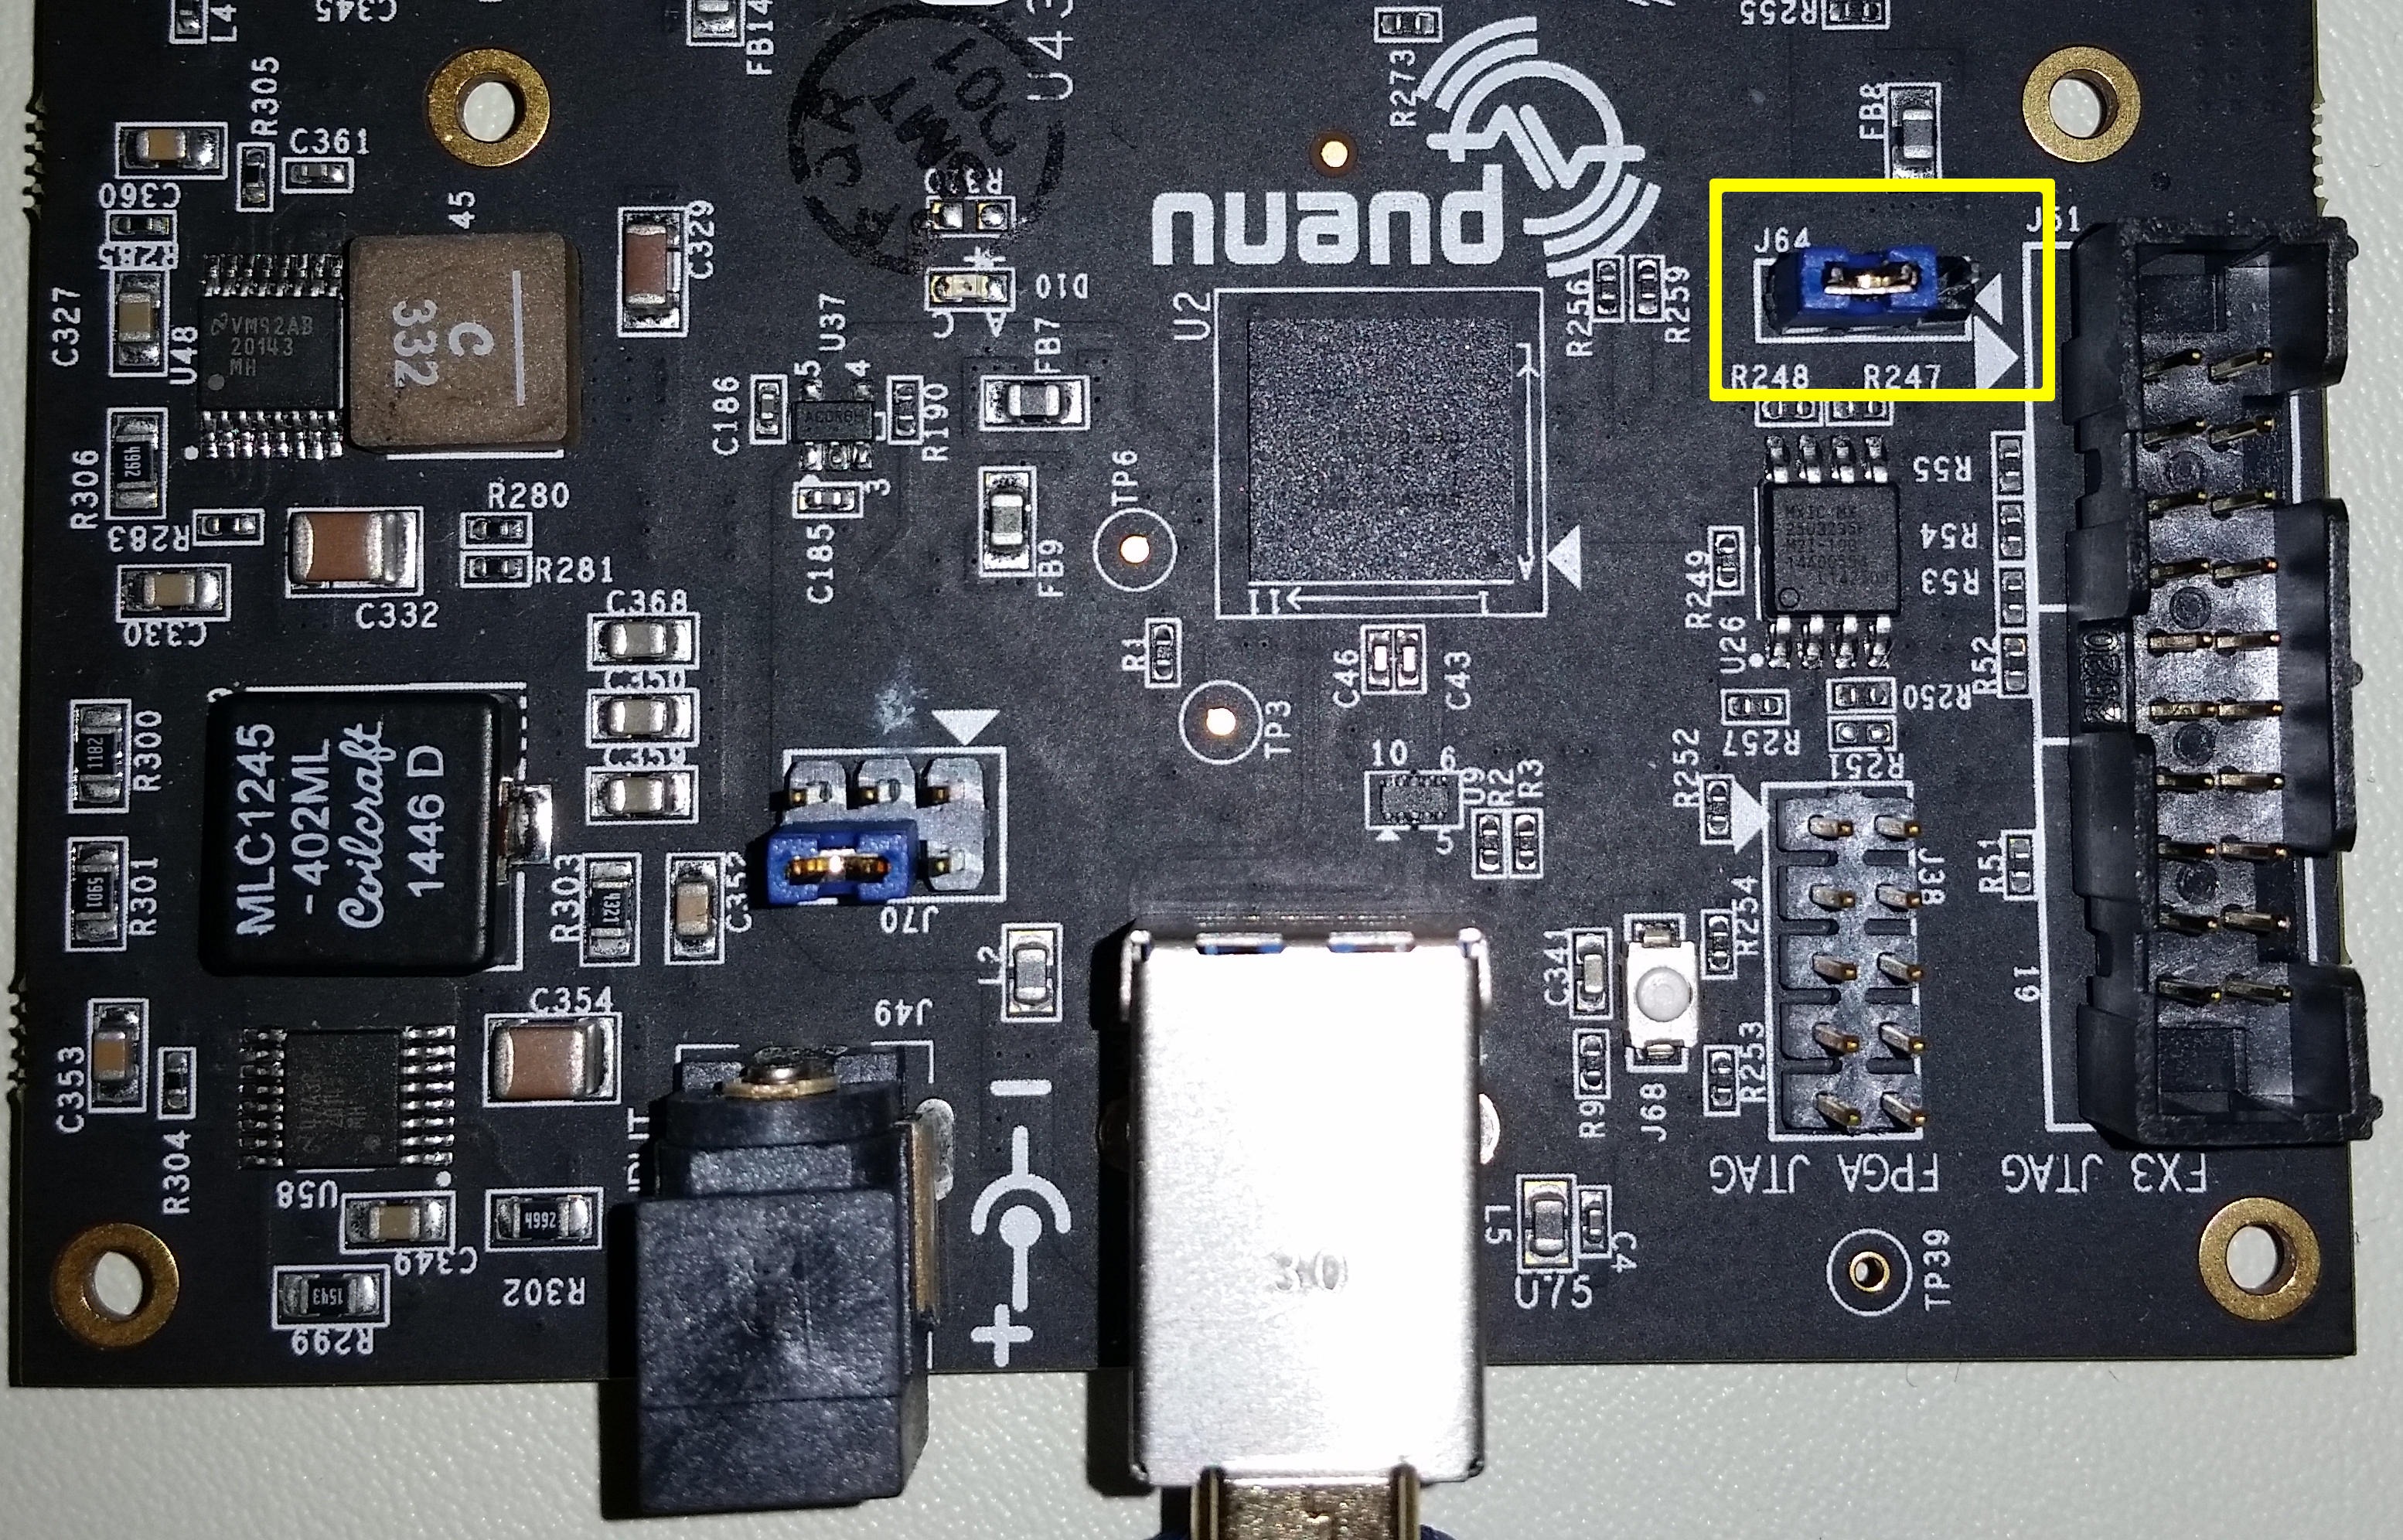
\includegraphics[width=4.5in]{images/bladeRF/j64-jumpered.jpg}
  \caption{bladeRF J64 jumper setting to force bootloader mode}
\end{figure}


To force the device into bootloader mode and re-flash firmware:
\begin{enumerate}
    \item Begin with the bladerf powered off.
    \item Place a jumper across pins 2 and 3 of header \texttt{J64}.
    \item Plug the device in to power it on.
    \item \textbf{Important}: Remove the jumper from \texttt{J64}.
        \begin{itemize}
            \item Forgetting this step will prevent the device from booting firmware in later steps.
        \end{itemize}
    \item Follow Section \ref{sec:recovery} to recover from the bootloader state
\end{enumerate}

\section{Troubleshooting} \label{sec:troubleshooting}

This section provides troubleshooting advice and solutions to common issues.

\subsection{Getting Help}\label{sec:help}

For issues not in this document, one may seek help through a number of other
avenues:

{\footnotesize
\begin{itemize}
    \item The \textit{Troubleshooting} forum \cite{TROUBLESHOOTING}
    \item IRC: \#bladeRF on Freenode \cite {FREENODE}
    \item Contacting Nuand
        \begin{itemize}
            \item \textit{Via email:} bladeRF@Nuand.com
            \item \textit{Via the Web:} \url{https://www.nuand.com/contact.php}
        \end{itemize}
\end{itemize}
}

\subsubsection{Information to Provide}
Below are some important of pieces of information to provide when asking
questions.

{\footnotesize
\begin{itemize}
    \item Information about the host machine
    \begin{itemize}
        \item Are you using a VM? What vitalization software and version?
        \item Are you using an embedded system, smartphone, or tablet? What specific device are you using?
        \item Are you using a USB 2.0 or USB 3.0 port? At which speed did the device connect?
        \item What USB host controller are you using?
    \end{itemize}

    \item Information about the host OS
    \begin{itemize}
        \item What version are you using? (\textit{\textbf{Linux users}: What distribution is it?})
        \item Is the OS 32-bit or 64-bit?
    \end{itemize}

     \item Software
     \begin{itemize}
         \item What \libbladerf, FPGA bitstream, and \fx3 firmware versions are in use?
         \item Where was the software obtained (\textit{e.g., from source, from a package manager})
         \item If using GNU Radio and/or gr-osmosdr, what are their corresponding versions?
     \end{itemize}

    \item Procedural issues
    \begin{itemize}
        \item What is the source of the procedure you are following? (\textit{e.g., website, guide, blog post, forum post})
        \item What steps have you already performed? Which one is causing issues?
    \end{itemize}

    \item Logs and Output
    \begin{itemize}
        \item Note any warnings or error messages.
        \item Gather verbose output from \bladerfcli using the \cmd{-v verobse} command-line option.
        \item Gather verbose output from \libbladerf-based programs by setting the \var{BLADERF\_LOG\_LEVEL} environment variable to \var{verbose}.
        \item \texttt{Linux Users:} Make a note of any relevant information in \cmd{dmesg} output.
    \end{itemize}
\end{itemize}
}

\subsection{Configuration and Build Issues}

\subsubsection{Warnings treated as errors}

By default, the host software is build with \texttt{-Werror} or \texttt{/WX},
with the intent of forcing developers and contributors to address warnings.

If you find that host software is not building due to a warning being treated
as an error, please contact the \bladerf developers to report this. Be sure
to accompany verbose build logs and your compiler version.

As a temporary workaround, you may configure the build to disable this behavior:
\begin{lstlisting}[style=snippet]
    cmake -DTREAT_WARNINGS_AS_ERRORS=OFF <path to CMakeLists.txt>
\end{lstlisting}

\subsubsection{Missing libusb}

\textit{\textbf{Linux and \osx}:}
If \cmake reports that libus is not found, it may be the case that
\program{pkg-config} could not find the library and/or its development headers.
Ensure the libusb development package has been installed and that the library
is in the standard library path or a location specified by the
\var{PKG\_CONFIG\_PATH} environment variable.

\textit{\textbf{\windows}:}
Verify that the \var{LIBUSB\_PATH} variable provided to \cmake is correctly assigned to
the location where libusb has been downloaded and extracted.

\subsubsection{Outdated libusb}

If the following message is printed when running \cmake, a newer libusb version
must be installed.

\begin{lstlisting}[style=snippet]
Failed to compile (compiled=0) or run (retval=255) libusb version check.
This may occur if libusb is earlier than v1.0.10.
Setting LIBUSB_VERSION to 0.0.0
\end{lstlisting}

libusb v1.0.10 or later is required to build. The latest available version is
\textbf{highly} recommended, due to numerous fixes and improvements (or added
support) for USB 3.0 and various OSes. See the libusb \fname{ChangeLog} file
\cite{LIBUSB_CHANGELOG} for more information.

\subsection{Runtime Issues}

\subsubsection{Unable to Find/Open Device: Linux}\label{sec:open-linux}

If unable to open the \bladerf in Linux, it may be the case that the current
user does not have sufficient permissions to access the device.

As of \libbladerf v1.5.0, a warning will be printed if this is the case and
associated API functions will return a status of \var{BLADERF\_ERR\_PERMISSION}.

\begin{lstlisting}[style=numbered-snippet, caption=Insufficient permissions to probe device]
$ bladeRF-cli -p

[WARNING @ libusb.c:292] Found a bladeRF via VID/PID, but could not open
                         it due to insufficient permissions.

  probe: No devices are available. If one is attached, ensure it
         is not in use by another program and that the current
         user has permission to access it.

\end{lstlisting}

\begin{lstlisting}[style=numbered-snippet, caption=Insufficient permissions to open device]
[WARNING @ libusb.c:428] Found a bladeRF via VID/PID, but could not open
                         it due to insufficient permissions.

No bladerf device(s) available.

If one is attached, ensure it is not in use by another program
and that the current user has permission to access it.
\end{lstlisting}

If using an older version, note that using running
\cmd{bladeRF-cli -v verbose} will print out more information about error codes,
and that setting \var{BLADERF\_LOG\_LEVEL=debug} in your environment will
provide additional debug output.

In order to access the \bladerf, Linux users must ensure:
%
\begin{itemize}
    \item The \fname{88-nuand.rules} file has been installed to \fname{/etc/udev/rules.d/}
    \item When building from source, the CMake option \var{INSTALL\_UDEV\_RULES} defaults to \var{ON}.
    \item The user is in the group specified by the CMake variable \var{BLADERF\_GROUP}.
\end{itemize}


The \var{BLADERF\_GROUP} defaults to \var{plugdev}, because Debian/Ubuntu users are
typically in this group when allowed to access removable USB storage devices.
You may wish to change this to conform to your security policies or
distribution.  The udev rules have been reloaded since the installation of the
aforementioned rules file. This can be done via executing the following
command and then re-plugging the device:

\centerline{\cmd{sudo udevadm control --reload-rules}}

If you have verified the above items and still cannot see the device:

\begin{itemize}
    \item Ensure the device is powered, as indicated by a lit LED \texttt{D1}.
    \item Confirm that you see the device in the output of \cmd{lsusb -v}
    \item Look for any information about the device's connection in the output
          \program{dmesg}
    \item Look for any failure messages in the log from the command:\\
          \cmd{bladeRF-cli -e version -v verbose}
    \item Examine and test the above for both USB 2.0 and USB 3.0 ports, if possible.
\end{itemize}

\subsubsection{Unable to Find/Open Device: \windows}\label{sec:open-windows}

To find and open the \bladerf in \windows, either a \libusb-based
driver or \cypress \cyusb driver must be installed. These drivers
may be installed using the \bladerf \windows installer
\cite{BLADERF_WINDOWS_INSTALL_GUIDE}. Alternatively, one may use \zadig
\cite{ZADIG} to install a \libusb-based driver.

Once a driver has been installed, ensure that the device is listed as
being associated with this driver in Device Manager. If this is the case
and the device still cannot be opened:

\begin{itemize}
    \item Ensure the device is powered, as indicated by a lit LED \texttt{D1}.
    \item Look for any failure messages in the log from the command:\\
          \cmd{\bladerf-cli -e version -v verbose}
    \item Examine and test the above for both USB 2.0 and USB 3.0 ports, if possible.
\end{itemize}

\subsubsection{Unable to Find/Open Device: \osx}\label{sec:open-osx}

If a device cannot be opened in \osx, first verify that the device is
powered on (which may be observed via LED \texttt{D1}) and is
is detected by the system:

\begin{lstlisting}[style=snippet, caption=\cmd{system\_profiler} output showing connected \bladerf]
$ system_profiler SPUSBDataType

USB:

    USB 3.0 Bus:

      Host Controller Driver: AppleUSBXHCIPPT
      PCI Device ID: 0x1e31
      PCI Revision ID: 0x0004
      PCI Vendor ID: 0x8086

        bladeRF:

          Product ID: 0x6066
          Vendor ID: 0x1d50
          Version: 0.00
          Serial Number: 9d1698a25946a1ce2876ab5953b45fb
          Speed: Up to 5 Gb/sec
          Manufacturer: Nuand
          Location ID: 0x14600000 / 10
          Current Available (mA): 1800
          Current Required (mA): 200
          Extra Operating Current (mA): 300

    USB 3.0 Bus:

      Host Controller Driver: AppleUSBXHCIPCI
      PCI Device ID: 0x1142
      PCI Revision ID: 0x0000
      PCI Vendor ID: 0x1b21
\end{lstlisting}

If the device appears in \cmd{system\_profiler} output:

\begin{itemize}
    \item Look for any failure messages in the log from the command:\\
          \cmd{bladeRF-cli -e version -v verbose}
      \item Look for any connection-related information in the output of: \cmd{sudo dmesg}
    \item Examine and test the above for both USB 2.0 and USB 3.0 ports, if possible.
    \item Reinstall \libusb from \macports or \brew. It has been reported that after
        performing a system upgrade, conflicts between the \osx \libusb and a version
        installed via \macports or \brew result in the inability to open a \bladerf.
        Reinstalling \libusb from the associated third-party package manager has
        been found to be a solution to this.
\end{itemize}

\subsubsection{Permissions Errors with PyBOMBS-based Install}\label{sec:open-linux}
\pybombs \cite{PYBOMBS} allow users to perform installations as non-root users.
To support this, it builds \bladerf support using the \cmake argument,
\var{-DINSTALL\_UDEV\_RULES=OFF}.  This prevents the installation from
attempting to copy \program{udev} rules to \fname{/etc/udev/rules.d/}.  As a
result, users may see the permissions errors
shown in Section \ref{sec:open-linux}.

Therefore, \pybombs users may need to (have their administrator) install the
\fname{88-nuand.rules} \cite{BLADERF_UDEV} file:

\begin{lstlisting}[style=numbered-snippet, caption=Manually installing udev rules]
# Download this file from the source repository
$ wget https://github.com/Nuand/bladeRF/blob/master/host/misc/udev/88-nuand.rules.in
$ mv 88-nuand-rules.in 88-nuand.rules

# Edit the file to replace @BLADERF_GROUP@ with a group your user is in.
$ vi 88-nuand.rules

# Change its permissions and install it
$ sudo chmod 644 88-nuand.rules
$ sudo mv 88-nuand.rules /etc/udev/rules.d/

# Reload the rules. Unplug and re-attach the device after running this.
$ sudo udevadm control --reload-rules
\end{lstlisting}

\subsubsection{Failure to Use Device on Embedded Platforms}

Some embedded platforms may not be able to supply a sufficient amount of
power to the \bladerf via the USB connection alone (especially on USB 2.0). The
symptoms of the device being underpowered vary. The device may
constantly enumerate in bootloader mode, or the device fails to open while
attempting to load its FPGA bitstream.

Therefore, when working with embedded platforms, it is recommended to either:
\begin{itemize}
    \item Use a USB 3.0 port, if available.
    \item Use an \textbf{externally powered} USB 3.0 hub.
    \item Power the \bladerf through its DC barrel jack instead of the USB connection.
\end{itemize}

\subsubsection{Multiple Programs Attempting to Access the Device}

\libbladerf allows only one process to access the device at any given time. If
an application unexpectedly reports that no \bladerf devices are available, ensure
that no applications are currently holding open device handles.

When applications are holding a handle to a \bladerf, \texttt{LED2} on the
\bladerf will blink. This provides a quick visual means of checking whether
another process was left using the device.

\subsubsection{Failures on USB 3.0 only}

If a \bladerf operates correctly on a USB 2.0 connection, but not on a USB 3.0
connection, it may be the case that: \begin{itemize}
    \item \textbf{\libusb}: A newer \libusb version may be required. See the
        \libusb CHANGELOG \cite{LIBUSB_CHANGELOG} for notes regarding USB 3.0
        support on your operating system.

    \item \textbf{Linux}: Driver or kernel updates may be required. For example,
        a 3.12 patch \cite{LINUX_SGLIMIT_PATCH} was reported to resolve
        FPGA-loading issues on USB 3.0 with certain host controllers.. Other
        fixes applied after the 3.13 kernel release reportedly fixed issues
        such as poor transfer rates and system-wide lockups when using a
        Renesase uPD720202-based
        controller.

    \item The USB 3.0 controller being used may require a firmware or driver
        update.  Early XHCI controllers are known to have a number of defects.
        Check the chipset or card manufacturer's website for updates.

        Should USB 3.0 issues be found to be associated to a particular chipset, it is
        recommended to upgrade to at \textit{least} an Intel 7 Series XHCI. (Later
        series have been found to yield improved perfomance.)

\end{itemize}

\subsubsection{libbladerf Messages About Outdated Firmware or FPGA}

\libbladerf will print warnings if it detects that either firmware executing on the \fx3
or the bitstream loaded in the FPGA are too old to allow for proper operation.

Additionally, \libbladerf will return the \var{BLADERF\_ERR\_SUPPORT} status
code when API functionality is not available with the firmware or FPGA version being
used. Enabling the debug log-level will often provide additional information in
this case.

See Section \ref{sec:fw-upgrade} for more information about upgrading the \fx3 firmware,
and the Nuand FPGA download page \cite{BLADERF_FPGA} for the latest FPGA version.

\subsubsection{Messages About Outdated libbladeRF}

\libbladerf prints one the following messages if the \fx3 firmware or FPGA bitstream
versions in use supersedes the version of libbladeRF that is in use:

\begin{lstlisting}[style=snippet]
    FPGA version (vX.Y.Z) is newer than entries in libbladeRF's compatibility table.
    Please update libbladeRF if problems arise.
\end{lstlisting}

\begin{lstlisting}[style=snippet]
    Firmware version (vX.Y.Z) is newer than entries in libbladeRF's compatibility table.
    Please update libbladeRF if problems arise.
\end{lstlisting}

This message is simply intended to let the user know that the firmware or FPGA
versions being used have been developed and tested with a newer version of \libbladerf.
In most cases, \libbladerf will operate successfully with newer versions of
these items. However, it is generally recommended to upgrade \libbladerf to
obtain fixes and new features.

\subsubsection{bladeRF-cli Reports Device is in Bootloader Mode}

When starting up, \bladerfcli detects devices in this bootloader mode
and prints a message alerting users to this: \\

\begin{lstlisting}[style=snippet]
    NOTE: One or more FX3-based devices operating in bootloader mode
          were detected. Run 'help recover' to view information about
          downloading firmware to the device(s).
\end{lstlisting}

See Section \ref{sec:recovery} for more information about recovering from
this state.

\subsubsection{Devices Times Out While Loading FPGA}

Attempting to load the wrong (or corrupted) FPGA image to the bladeRF results
in \libbladerf returning the \var{BLADERF\_ERR\_TIMEOUT} status code. Verify
that you are using the correct image for your device.

If you are unsure as to which size FPGA is on your \bladerf, identify the
Altera Cyclone IV package on the top of the \bladerf. The chip package should
read \textit{EP4CExF23C8N}, where \textit{x} is either 40 or 115. Use the
\fname{hostedx40.rbf} file for the former, and \fname{hostedx115.rbf} for the latter.

\subsubsection{Failure to find libbladeRF.so, libbladeRF.dylib, or bladeRF.dll}

If a program fails to run, printing a message that \fname{libbladeRF.so} (Linux),
\fname{libbladeRF.dylib} (OSX), or \fname{bladeRF.dll} (\windows) cannot be found,
it may be the case that the system does not have \libbladerf in its library search path.

\textbf{Linux and OSX}:
If you have build \bladerf software from source, but are unsure where it has
been installed, refer to the \fname{install\_manifest.txt} file within your
build directory, and/or the \var{CMAKE\_INSTALL\_PREFIX} variable in
\fname{CMakeCache.txt}

\textbf{Linux}: \\
Ensure that \libbladerf is installed in a location specified in one of the files
in \fname{/etc/ld.so.conf.d/} or create a new file in this directory specifying the
location of \libbladerf. Check the output of \program{ldd <your program>} to
determine where the program is attempting to find \libbladerf. Using
\var{LD\_LIBRARY\_PATH} may be helpful in debugging library path issues, but
is not recommended as a permanent solution.


\textbf{\osx}: \\
Generally, applications in OSX utilize \texttt{@rpath} to establish paths to
shared libraries. Use \cmd{otool -L <your program>} to check the location where
the program is attempting to find \libbladerf. Using \var{DYLIB\_LIBARARY\_PATH}
may be helpful in debugging library path issues, but is not recommended as a
permanent solution.

\textbf{\windows}: \\
Ensure that the folder containing \program{bladeRF.dll} is listed in the \var{PATH}
environment variable. If you have updated \var{PATH} (either manually or via the
\bladerf installer), you may need to log out and log back in before the change
takes effect.


\newpage
{\footnotesize \bib}
\end{document}
